\documentclass[10pt,a4paper,twocolumn]{article}
\usepackage[utf8]{inputenc}
\usepackage[T1]{fontenc}
\usepackage[brazil]{babel}
\usepackage{geometry}
\geometry{left=1.6cm,right=1.6cm,top=1.45cm,bottom=1.45cm}
\usepackage{amsmath,graphicx,booktabs,microtype}
\usepackage{listings,xcolor}
\usepackage{float}
\setlength{\columnsep}{0.62cm}
\setlength{\parindent}{0.85em}
\setlength{\parskip}{0pt}
\newcommand{\tppseparador}{\vspace{0.5em}}
\title{\vspace{-1.4cm}\bfseries\normalsize TPP4: Simula\c{c}\~ao Paralela da Propaga\c{c}\~ao de Inc\^endios Florestais}
\author{\small [Integrantes do grupo] \\ \small Computa\c{c}\~ao Paralela --- PUCRS --- Prof. C\'esar A. F. De Rose}
\date{\vspace{-0.8cm}}
\begin{document}
\maketitle
\vspace{-1.4em}
\noindent\textbf{Objetivo.} Investigar o desempenho do modelo de \emph{fases paralelas}, comparando MPI puro e MPI+OpenMP na simula\c{c}\~ao de inc\^endios florestais em quatro n\'os da Atl\^antica.

\section*{Modelo e implementa\c{c}\~ao}
A floresta corresponde a uma matriz bidimensional, cujas c\'elulas assumem quatro estados: solo, vegeta\c{c}\~ao, fogo e queimada. Inicialmente, a cobertura vegetal \`e definida por um gerador determin\'istico por coordenada, com foco de igni\c{c}\~ao central. Em cada passo, o estado de uma c\'elula depende dos seus oito vizinhos; fontes a oeste recebem maior peso, simulando vento para leste. Cada c\'elula em chamas passa a queimada no passo seguinte.

A grade foi decomposta em faixas horizontais cont\'iguas de igual tamanho (uma por \emph{rank}). O algoritmo repete: (1) atualiza\c{c}\~ao paralela de cada faixa; (2) \texttt{MPI\_Allreduce} para somar as c\'elulas em chamas e identificar extin\c{c}\~ao; (3) \texttt{MPI\_Sendrecv} para atualizar as duas linhas de fronteira com os processos vizinhos. Uma troca inicial prepara as bordas antes da primeira atualiza\c{c}\~ao. A execu\c{c}\~ao encerra por extin\c{c}\~ao ou por limite fixo de passos. No modo h\'ibrido, \texttt{\#pragma omp parallel for} divide as linhas locais entre as threads; somente a thread principal invoca MPI (\texttt{MPI\_THREAD\_FUNNELED}).

\section*{Metodologia experimental}
Os experimentos utilizam \textbf{4 n\'os} da Atl\^antica, com \textbf{8 n\'ucleos f\'isicos (16 threads l\'ogicas) por n\'o}. Comparam-se duas quantidades de trabalhadores (32 e 64) e duas organiza\c{c}\~oes por quantidade, usando a mesma entrada, semente e limite de itera\c{c}\~oes. Cada configura\c{c}\~ao \`e executada tr\^es vezes, alternando-se a ordem dos cen\'arios. O tempo informado \`e o maior tempo por processo MPI, incluindo processamento, coletivas e troca de bordas (sem inicializa\c{c}\~ao nem gera\c{c}\~ao de imagens). Valida-se a equival\^encia dos resultados pela assinatura global, contagens de estados e n\'umero de passos.

\begin{table}[H]
\centering\small
\caption{Configura\c{c}\~oes previstas. HT: Hyper-Threading.}
\begin{tabular}{@{}lrrl@{}}
\toprule
Vers\~ao & MPI & Threads/rank & Total\\
\midrule
MPI puro & 32 & 1 & 32\\
MPI+OpenMP & 4 & 8 & 32\\
MPI puro (HT) & 64 & 1 & 64\\
MPI+OpenMP (HT) & 4 & 16 & 64\\
\bottomrule
\end{tabular}
\end{table}

\section*{Resultados e discuss\~ao}
\begin{table}[H]
\centering\small
\caption{Tempo total em segundos: m\'edia e desvio-padr\~ao de $n$ execu\c{c}\~oes.}
\begin{tabular}{@{}lrrr@{}}
\toprule
Configura\c{c}\~ao & M\'edia & DP & $n$\\
\midrule
\IfFileExists{resultados/tabela_resultados.tex}{\input{resultados/tabela_resultados.tex}}{%
MPI 32 & -- & -- & --\\
H\'ibrido 4$\times$8 & -- & -- & --\\
MPI 64 (HT) & -- & -- & --\\
H\'ibrido 4$\times$16 (HT) & -- & -- & --\\
}
\bottomrule
\end{tabular}
\end{table}

\noindent\textbf{An\'alise a completar com dados reais:} calcular $T_{\text{MPI32}}/T_{\text{H4x8}}$ e $T_{\text{MPI64}}/T_{\text{H4x16}}$; explicar poss\'iveis ganhos da redu\c{c}\~ao de \emph{ranks} e da comunica\c{c}\~ao entre fronteiras, e perdas com sincroniza\c{c}\~ao e HT. Relatar a grade, os passos executados e se o fogo extinguiu ou se atingiu o limite. \textbf{N\~ao preencher sem execu\c{c}\~oes reais.}

\begin{figure}[H]
\centering
\IfFileExists{figuras/comparativo_tempos.png}{%
\includegraphics[width=0.99\columnwidth]{figuras/comparativo_tempos.png}
\caption{Compara\c{c}\~ao de tempos reais das quatro configura\c{c}\~oes.}
}{%
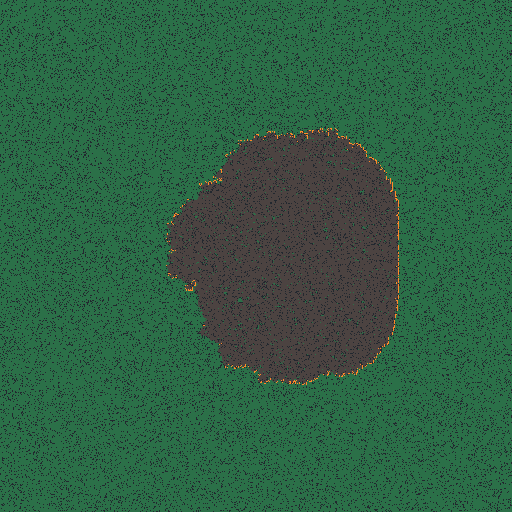
\includegraphics[width=0.81\columnwidth]{figuras/incendio_exemplo_fim.png}
\caption{Estado ilustrativo ap\'os 140 passos em grade $512\times512$ (teste local, n\~ao \`e benchmark MPI).}
}
\end{figure}

\section*{Conclus\~ao}
O modelo permite separar o custo de atualiza\c{c}\~ao local e o custo da comunica\c{c}\~ao. \textbf{Preencher ap\'os os testes:} indicar qual configura\c{c}\~ao foi mais r\'apida, o efeito do HT e a explica\c{c}\~ao causal para os resultados observados.

\section*{Refer\^encias e uso de IA}
Manuais Open MPI (\texttt{MPI\_Allreduce}, \texttt{MPI\_Sendrecv}) e SchedMD (\texttt{srun}); C++17, MPI, OpenMP, Slurm e Python; ferramentas de IA generativa auxiliaram na estrutura\c{c}\~ao do c\'odigo, na valida\c{c}\~ao e na reda\c{c}\~ao, com revis\~ao e execu\c{c}\~ao sob responsabilidade do grupo.

\clearpage
\onecolumn
\appendix
\section*{Ap\^endice A --- C\'odigo-fonte integral com linhas numeradas}
\lstset{
 basicstyle=\ttfamily\scriptsize,
 keywordstyle=\color{blue!55!black},
 commentstyle=\color{gray!75!black},
 stringstyle=\color{green!40!black},
 numbers=left,numberstyle=\tiny\color{gray},stepnumber=1,
 numbersep=7pt,frame=single,breaklines=true,breakatwhitespace=false,
 keepspaces=true,columns=fullflexible,showstringspaces=false,
 tabsize=4,language=C++
}
\lstinputlisting{incendio.cpp}
\end{document}
